\section{Citations}
\label{sec: citations}

In this section, a \emph{very} rough explanation on how biliographies and their implementation work in LaTeX will be given. This is not a comprehensive guide, but rather a quick overview.

In LaTeX, BibTeX is often used to describe various distinct aspects, which can lead to confusion. Some reference BibTeX as the program that LaTeX uses to compile the bibliography, while others refer to compilation of the file. Then there's the integration of a the backend that is used to compile; \texttt{bibtex} and \texttt{biber}, and what those represent.

To start, there are two main distinctions in the bibliography process: the \emph{external programs} that process bibliography information, and roughly act as the middle-man between your \texttt{.bib} file and the LaTeX document, and the LaTeX \emph{packages} that you import into your compilation to handle the formatting of your citations and bibliography. Here is a simple view of the process:

\begin{figure}[h!]
    \centering
    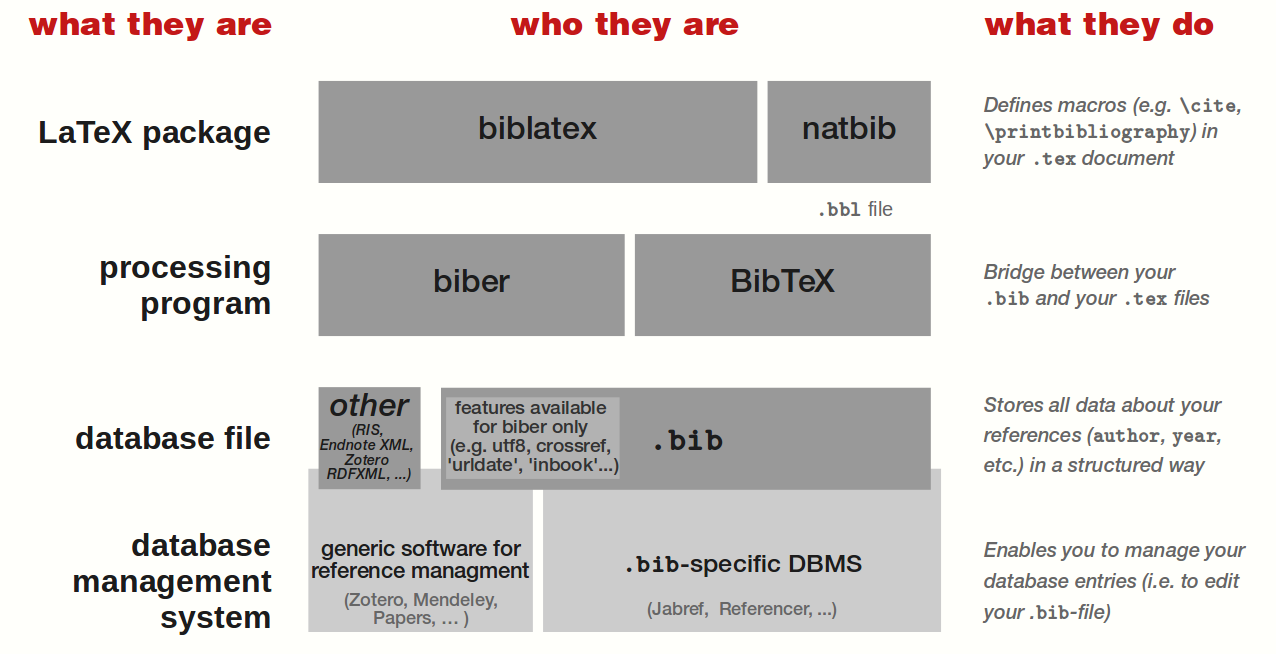
\includegraphics[width=0.8\textwidth]{content/citations_overview.png}
    \caption{Bibliography Process Overview in LaTeX}
    \label{fig: bibliography-process}
\end{figure}

At the highest level, there are two main front-end LaTeX packages that users interact with to handle citations, references, and bibliographies. These are \texttt{natbib} and \texttt{biblatex}. \texttt{natbib} is an older package, and although still maintained, may not be further developed. Despite this reasons, it is still widely used, and very reliable in nature. 
\texttt{biblatex} is a newer package that is more flexible and can handle more complex bibliography styles, and happens to be actively developed alongside the \texttt{biber} processing program (backend, more on this below). The humanities fields tend to use \texttt{biblatex} as many predefined styles are available (e.g., APA, MLA, Chicago). Science fields tend to go either way depending on the publishing journal's requirements and specific functionalities needed.

The backend or processing programs are the bridge between the LaTeX document and the bibliography file. The two main programs are \texttt{bibtex} and \texttt{biber}. \texttt{bibtex} interfaces with with specific \texttt{.bst} files, which are postfix language files that define the formatting of the bibliography. In the case of many major publication journals (especially in astronomy), the submission of manuscripts require the use of these \texttt{.bst} files, and as such, users are required to use the \texttt{natbib} LaTeX package. \texttt{biber} on the other hand is a relatively newer processing program that adds further functionality to \texttt{biblatex}.

It is important to note that the \texttt{biblatex} package can make use of either the \texttt{biber} backend or the \texttt{bibtex} backend, while the \texttt{natbib} package is restricted to the \texttt{bibtex} backend. Even more importantly, results with \texttt{biblatex} can differ depending on the backend: if \texttt{bibtex} is used, it only uses it for sorting, and not for formatting content.

The takeaways are the following: if you enjoy a particular style given in a particular journal, download it's \texttt{.bst} file and make use of the \texttt{natbib} package to compile your thesis work. In the case of this example PDF, the \texttt{aasjournal.bst} file is loaded, and it's style used in the bibliography:

\begin{lstlisting}[language=TeX]
    \TOCadd{Bibliography} % add citations to TOC
    \bibliography{AstroCitations.bib}{}
    \bibliographystyle{aasjournal} % links to aasjournal.bst file
\end{lstlisting}

A citation example is given here \citep{Hubble1929}.
